\chapter{BULGULAR VE TARTIŞMA}

Basit iki terimle \acrfull{lbp} ve \acrfull{hog} kısaltmaları anlatabiliriz. İster kısaltmasını \acrshort{lbp}, isterseniz de uzun açılımını \acrlong{hog} yazdırabilirsiniz. Bunu yapabilmek için dosyanın başında terimleri tanımlamanız gereklidir. İsterseniz matematik terimlerini de, örneğin \acrshort{fer} böyle tanımlayabilirsiniz. Uzun uzun \acrfull{fer} yazmanız gerekmez. 

\lipsum[19-25]

\section{section-name-1}

Öznitelik vektörleri oluşturulurken öncelikli olarak imge üzerinden yüz tespit edilmesi ve yüz üzerine 68 nirengi noktasının yerleştirmesiyle başlamıştır. Devam eden alt bölümlerde bu nirengi noktalarının görünüm ve geometrik olarak nasıl kullanıldığına yer verilecektir.

\subsection{subsection-name-1}

Eşitlik-\ref{eq:result_geo}’de verilen formüle 
\lipsum[2]


%eşitlik.
\begin{equation}
F_{x } =2 \times \frac{(n_{1})\times(n_{1}-1)}{2}  
\label{eq:result_geo}%
\end{equation}

\subsection{subsection-name-2}

\acrfull{hog} 
\lipsum[30]

%eşitlik.
\begin{equation}
F_{ x } = ((s_{row}/b_{row}) - c_{row} +1) \times ((s_{col} / b_{col}) - c_{col} +1) \times c_{row} \times c_{col} \times y
\label{eq:result_hog}%
\end{equation}


\subsection{subsection-name-3}

\acrlong{lbp} \lipsum[3]
%eşitlik.
\begin{equation}
F_{ \text{THETA} } = (n_{1} \times n_{2})
\label{eq:result_lbp}%
\end{equation}

\section{section-name-2}

\lipsum[22-25]
Tablo-\ref{tab:featuresize} de verilmiştir. 

\begin{table}[hpb]
    \centering
    \caption{Öznitelik çıkarım yöntemine göre boyut indirgenmiş öznitelik sayıları}
    \begin{tabular}{ |p{4.5cm}||p{2.5cm}|p{2.5cm}|p{2.5cm}|  }
     \hline
     \multicolumn{4}{|c|}{Öznitelik Sayıları} \\
     \hline
     Öznitelik Seçim Yöntemi& Geometrik & YGH & YİÖ\\
     \hline
     Temel Öznitelikler   & 1122    &2800&   17408\\
     \acrshort{sffs} &   60  & 171   &7680\\
     \acrshort{sbfs} & 28 & 195&  5888\\
     \acrshort{pca} & 268 & 268&  866\\
     \hline
    \end{tabular}
    \label{tab:featuresize}
\end{table}

\lipsum[3]

\section{section-name-3}

\lipsum[1-2]

\section{Deney Sonuçları}


 Çizelge-\ref{tab:smotetablo}'de 
 \lipsum[3]

\subsection{Final-Subsection-1}

Geometrik öznitelikleri için \acrshort{svm}, \acrshort{rf} ve \acrshort{logreg} sınıflandırıcıları ile sınıflandırma sonuçları  Şekil-\ref{fig:ckrawgeoall}'te verilmiştir. 

\begin{figure}[hbt!]

\begin{subfigure}{.475\linewidth}
  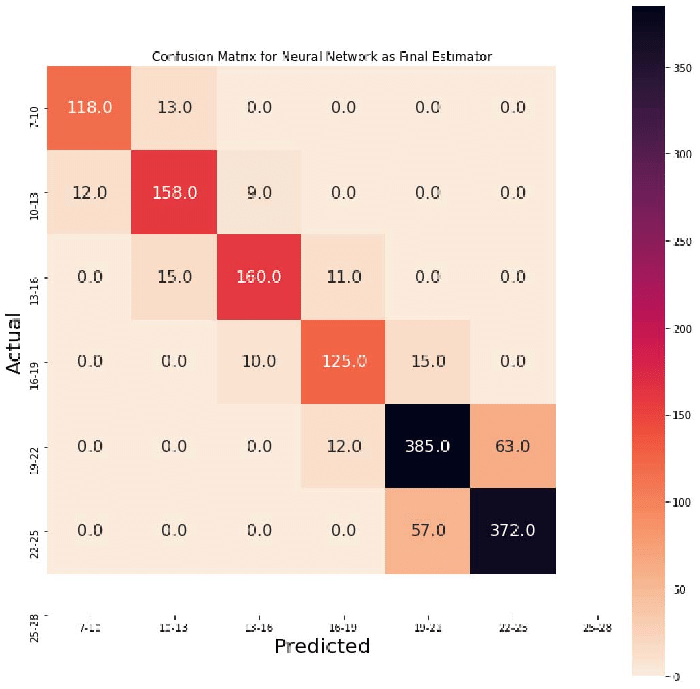
\includegraphics[trim={0 0 0 0.72cm},clip,width=\linewidth]{gorseller/Confusion-Matrix.png}
  \caption{DVM-$rbf$}
  \label{MLEDdet0}
\end{subfigure}\hfill % <-- "\hfill"
\begin{subfigure}{.475\linewidth}
  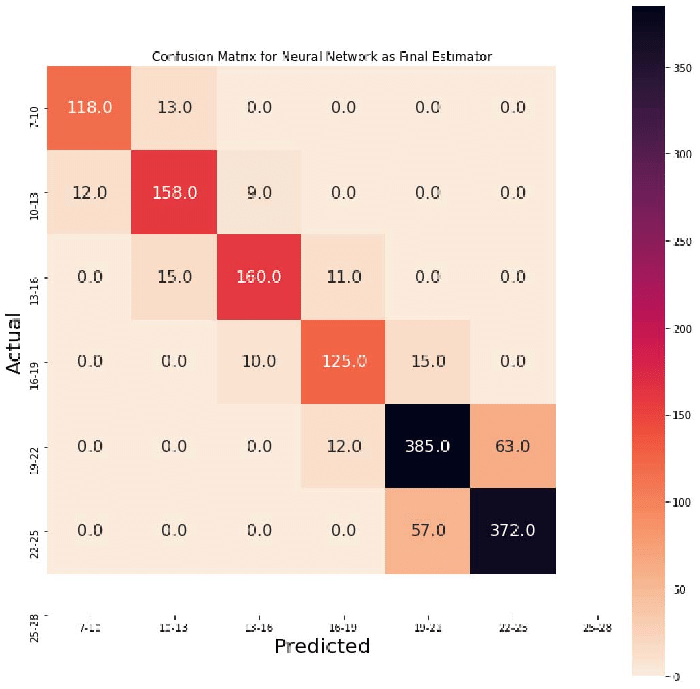
\includegraphics[trim={0 0 0 0.72cm},clip,width=\linewidth]{gorseller/Confusion-Matrix.png}
  \caption{DVM-$\textit{doğrusal}$}
  \label{energydetPSK0}
\end{subfigure}

\medskip % create some *vertical* separation between the graphs
\begin{subfigure}{.475\linewidth}
  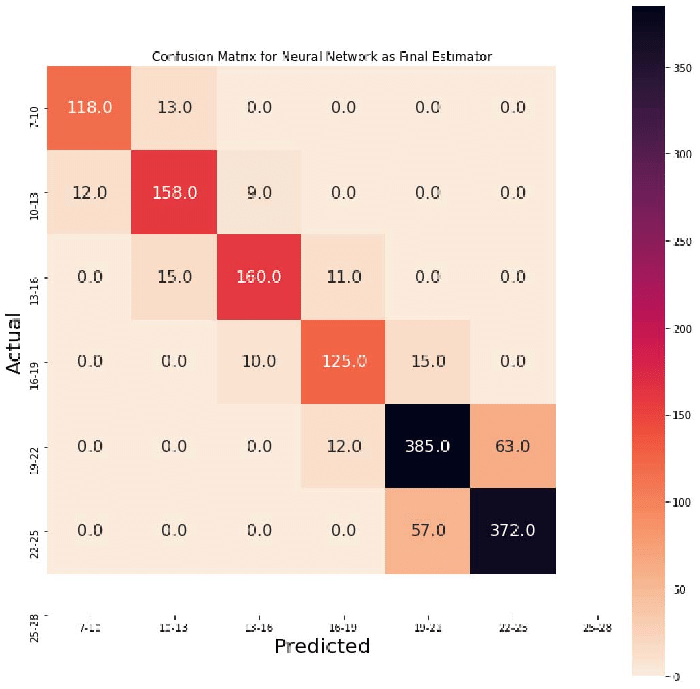
\includegraphics[trim={0 0 0 0.72cm},clip,width=\linewidth]{gorseller/Confusion-Matrix.png}
  \caption{RO}
  \label{velcomp0}
\end{subfigure}\hfill % <-- "\hfill"
\begin{subfigure}{.475\linewidth}
  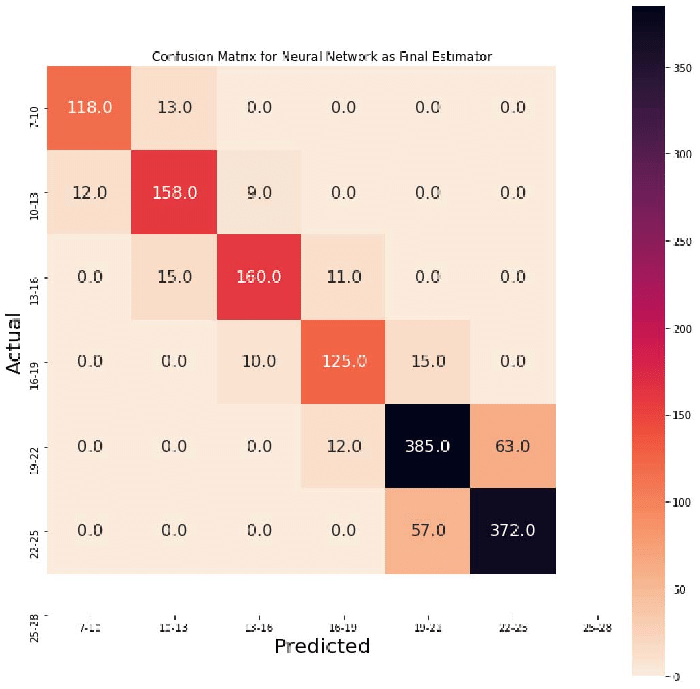
\includegraphics[trim={0 0 0 0.72cm},clip,width=\linewidth]{gorseller/Confusion-Matrix.png}
  \caption{LRC}
  \label{estcomp0}
\end{subfigure}

\caption{tab 2}
\label{fig:ckrawgeoall}
\end{figure}


\lipsum[4] 
Şekil-\ref{fig:ckrawgeoall}'te yer verilmiştir.

%Ssad


\begin{figure}[hbt!]

\begin{subfigure}{.475\linewidth}
  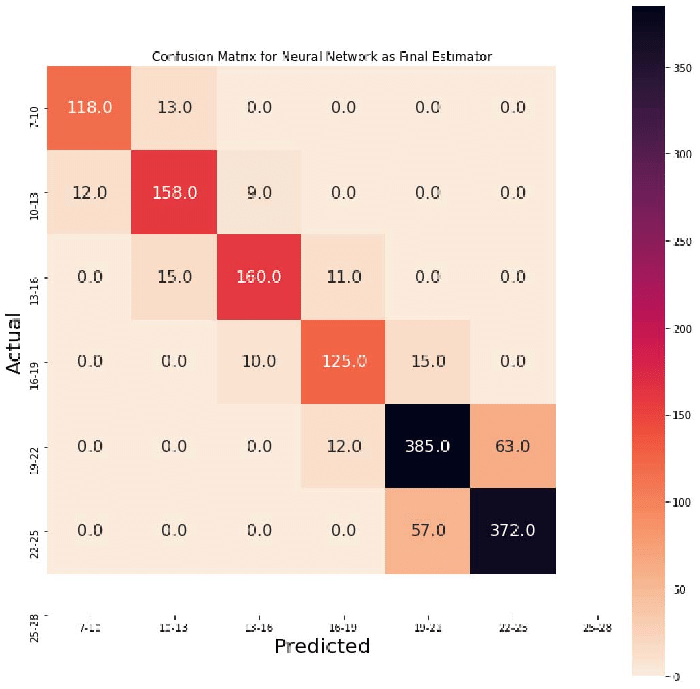
\includegraphics[trim={0 0 0 0.72cm},clip,width=\linewidth]{gorseller/Confusion-Matrix.png}
  \caption{DVM-$rbf$}
  \label{MLEDdet1}
\end{subfigure}\hfill % <-- "\hfill"
\begin{subfigure}{.475\linewidth}
  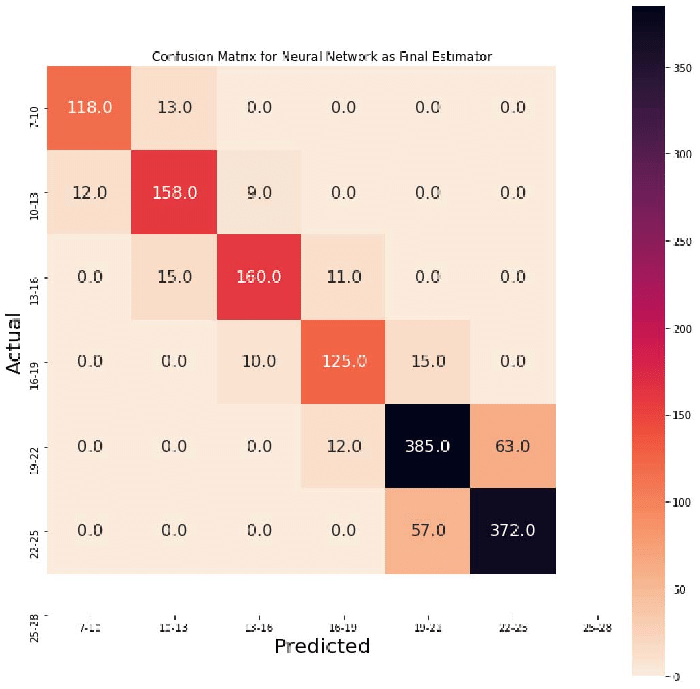
\includegraphics[trim={0 0 0 0.72cm},clip,width=\linewidth]{gorseller/Confusion-Matrix.png}
  \caption{DVM-$\textit{doğrusal}$}
  \label{energydetPSK1}
\end{subfigure}

\medskip % create some *vertical* separation between the graphs
\begin{subfigure}{.475\linewidth}
  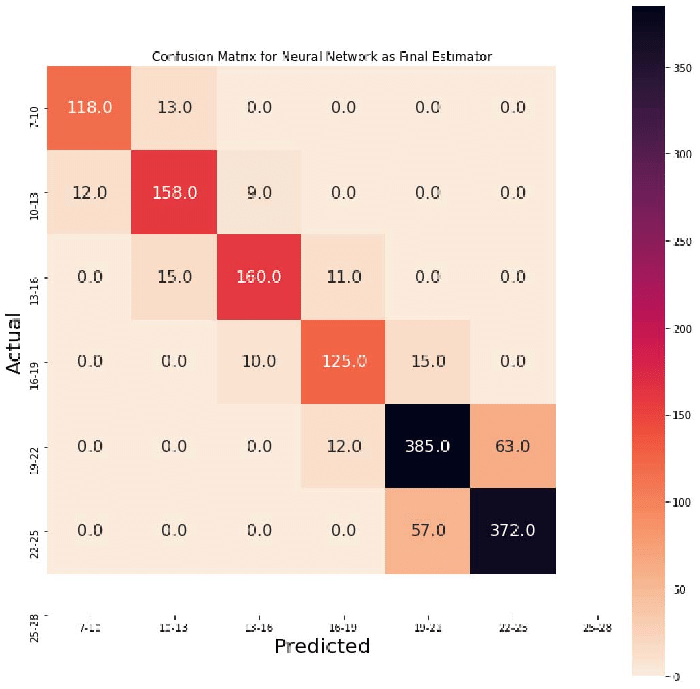
\includegraphics[trim={0 0 0 0.72cm},clip,width=\linewidth]{gorseller/Confusion-Matrix.png}
  \caption{RO}
  \label{velcomp1}
\end{subfigure}\hfill % <-- "\hfill"
\begin{subfigure}{.475\linewidth}
  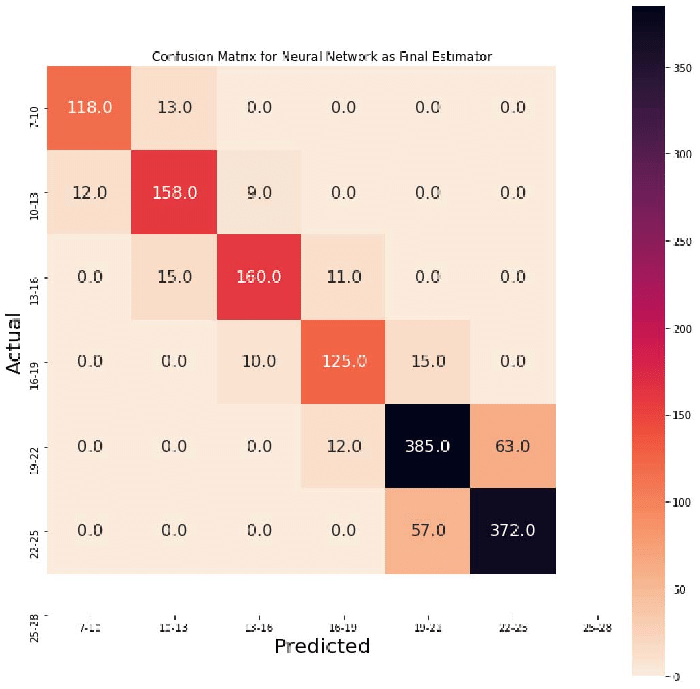
\includegraphics[trim={0 0 0 0.72cm},clip,width=\linewidth]{gorseller/Confusion-Matrix.png}
  \caption{LRC}
  \label{estcomp1}
\end{subfigure}

\caption{sdaafsfa}
\label{fig:cksffsgeoall}
\end{figure}

% \begin{figure}[hbp]
% \centering
% \includegraphics[trim={0 0 0 0.72cm},clip,width=0.53\textwidth]{conf_mat/conf_mat_geometric_sffs_rbf_SVM.png}
% \caption{AİÖS uygulanmış geometrik özniteliklerin DVM-$rbf$ çekirdeğindeki karmaşıklık matrisi}\label{fig:conf_mat_geometric_sffs_rbf_SVM}
% \end{figure}

% \begin{figure}[hp]
% \centering
% \includegraphics[trim={0 0 0 0.72cm},clip,width=0.53\textwidth]{conf_mat/conf_mat_geometric_sffs_Linear_SVM.png}
% \caption{AİÖS uygulanmış geometrik özniteliklerin DVM-$\textit{doğrusal}$ çekirdeği ile karmaşıklık matrisi}\label{fig:conf_mat_geometric_sffs_Linear_SVM}
% \end{figure}

% \begin{figure}[hp]
% \centering
% \includegraphics[trim={0 0 0 0.72cm},clip,width=0.53\textwidth]{conf_mat/conf_mat_geometric_sffs_Random_Forest.png}
% \caption{AİÖS uygulanmış geometrik özniteliklerin RO ile  karmaşıklık matrisi}\label{fig:conf_mat_geometric_sffs_Random_Forest}
% \end{figure}

% \begin{figure}[hp]
% \centering
% \includegraphics[trim={0 0 0 0.72cm},clip,width=0.53\textwidth]{conf_mat/conf_mat_geometric_sffs_Logistic_Regression.png}
% \caption{AİÖS uygulanmış geometrik özniteliklerin LRS ile karmaşıklık matrisi}\label{fig:conf_mat_geometric_sffs_Logistic_Regression}
% \end{figure}



% \begin{figure}[hbp]
% \centering
% \includegraphics[trim={0 0 0 0.72cm},clip,width=0.53\textwidth]{conf_mat/conf_mat_geometric_sbfs_rbf_SVM.png}
% \caption{AGÖS uygulanmış geometrik özniteliklerin DVM-$rbf$ çekirdeğindeki karmaşıklık matrisi}\label{fig:conf_mat_geometric_sbfs_rbf_SVM}
% \end{figure}

% \begin{figure}[hp]
% \centering
% \includegraphics[trim={0 0 0 0.72cm},clip,width=0.53\textwidth]{conf_mat/conf_mat_geometric_sbfs_Linear_SVM.png}
% \caption{AGÖS uygulanmış geometrik özniteliklerin DVM-$\textit{doğrusal}$ çekirdeği ile karmaşıklık matrisi}\label{fig:conf_mat_geometric_sbfs_Linear_SVM}
% \end{figure}

% \begin{figure}[htbp]
% \centering
% \includegraphics[trim={0 0 0 0.72cm},clip,width=0.53\textwidth]{conf_mat/conf_mat_geometric_sbfs_Random_Forest.png}
% \caption{AGÖS uygulanmış geometrik özniteliklerin RO ile  karmaşıklık matrisi}\label{fig:conf_mat_geometric_sbfs_Random_Forest}
% \end{figure}

% \begin{figure}[htbp]
% \centering
% \includegraphics[trim={0 0 0 0.72cm},clip,width=0.53\textwidth]{conf_mat/conf_mat_geometric_sbfs_Logistic_Regression.png}
% \caption{AGÖS uygulanmış geometrik özniteliklerin LRS ile karmaşıklık matrisi}\label{fig:conf_mat_geometric_sbfs_Logistic_Regression}
% \end{figure}

% \lipsum[1]

% \begin{figure}[htbp]
% \centering
% \includegraphics[trim={0 0 0 0.72cm},clip,width=0.53\textwidth]{conf_mat/conf_mat_geometric_pca_rbf_SVM.png}
% \caption{TBA öznitelik seçimi uygulanmış geometrik özniteliklerin DVM-$rbf$ çekirdeğindeki karmaşıklık matrisi}\label{fig:conf_mat_geometric_pca_rbf_SVM}
% \end{figure}

% \begin{figure}[htbp]
% \centering
% \includegraphics[trim={0 0 0 0.72cm},clip,width=0.53\textwidth]{conf_mat/conf_mat_geometric_pca_Linear_SVM.png}
% \caption{TBA öznitelik seçimi uygulanmış geometrik özniteliklerin DVM-$\textit{doğrusal}$ çekirdeği ile karmaşıklık matrisi}\label{fig:conf_mat_geometric_pca_Linear_SVM}
% \end{figure}

% \begin{figure}[htbp]
% \centering
% \includegraphics[trim={0 0 0 0.72cm},clip,width=0.53\textwidth]{conf_mat/conf_mat_geometric_pca_Random_Forest.png}
% \caption{TBA öznitelik seçimi uygulanmış geometrik özniteliklerin RO ile  karmaşıklık matrisi}\label{fig:conf_mat_geometric_pca_Random_Forest}
% \end{figure}

% \begin{figure}[htbp]
% \centering
% \includegraphics[trim={0 0 0 0.72cm},clip,width=0.53\textwidth]{conf_mat/conf_mat_geometric_pca_Logistic_Regression.png}
% \caption{TBA öznitelik seçimi uygulanmış geometrik özniteliklerin LRS ile karmaşıklık matrisi}\label{fig:conf_mat_geometric_pca_Logistic_Regression}
% \end{figure}


\clearpage
\newpage
\lipsum[5]
Çizelge-\ref{tab:ckgeometrikacc}'de verilmiştir. 
\lipsum[6]



\begin{table}[hpt]
    \centering
    \caption{sınıflandırma Sonuçları}
    \begin{tabular}{ |p{3cm}||p{3cm}|p{2.5cm}|p{2.5cm}|  }
     \hline
     \multicolumn{4}{|c|}{ ccccccc test} \\
     \hline
     \hline
     feats & cccccc &X1 & X2\\
     \hline
     \hline
     \multirow{5}{4em}{feat3} & XXX-$\textit{ll}$ & 0.8821 &	0.9836 \\ 
         & ddd-$rbf$ & 0.8474 &	0.9570
  \\ 
         & rrr & 0.7782&	0.9423
 \\ 
         & lll & 0.9145	&\textbf{0.9854}
 \\ 
         & ooo & 0.6982&	0.9250
\\
     \hline
     \multirow{5}{4em}{feat2} & XXX-$\textit{ll}$ & 0.8695&	0.9639
\\ 
         & ddd-$rbf$ & 0.8915&	0.9544
 \\ 
         & rrr & 0.8048&	0.9381
\\ 
         & lll & 0.8834&	0.9621
\\ 
         & ooo & 0.8236	&0.9232
\\
     \hline
     \multirow{5}{4em}{feat1} & XXX-$\textit{ll}$ & 0.9272&	0.9803
\\ 
         & ddd-$rbf$ & \textbf{0.9352}&	0.9578
\\ 
         & rrr & 0.7991&	0.9382
\\ 
         & lll & 0.9157&	0.9750
\\ 
         & ooo & 0.8375&	0.8991
\\
     \hline
     \multirow{5}{4em}{feat} & XXX-$\textit{ll}$ & 0.8901&	0.9845
\\ 
         & ddd-$rbf$ & 0.8326&	0.9527
 \\ 
         & rrr & 0.8060&	0.9441
\\ 
         & lll & 0.9086&	0.9837
\\ 
         & ooo & 0.7169&	0.9384
\\
     \hline
    \end{tabular}
    \label{tab:ckgeometrikacc}
\end{table}


\subsection{Final-Subsection-2}

\lipsum[1-2]



% ==========================================

% ==========================================
\subsection{Final-Subsection-3}

\lipsum[4-6]



% ====================================

\subsection{Final-Subsection-4}
\lipsum[10-11]
% ===========================================================================
% ===========================================================================
% ===========================================================================
\newpage
\subsection{Final-Subsection-5}
\lipsum[12-13]